\newcommand\mybox[2][]{\tikz[overlay]\node[fill=lightyellow,inner sep=2pt, anchor=text, rectangle, rounded corners=1mm,draw=black,#1] {#2};\phantom{#2}}

\tikzstyle{reddot}=[draw=black,line width=1pt,minimum size=1.5mm,inner sep=0pt,outer sep=0pt,shape=circle,fill=blue]
\tikzstyle{bluedot}=[draw=blue,minimum size=0.5mm,inner sep=0pt,outer sep=0pt,shape=circle,fill=blue]

%%%%%%%%%%%%%%%%%%%%%%%%%%%%%%%%%%%%%%%%%%%%%%%%%%%%%%%%%%%%%%%%%%%%%%%%%%%%%%%%
\begin{frame}{How structured is a metric space?}

%Many ways to measure (equilateral, Minkowski-Bouligand, Hausdorff, ...)
That is, what is it's dimension?

\pause
\vspace{0.1in}
We'll use the \emph{doubling dimension} $c$
 
\pause
\vspace{0.1in}
Captures the idea of an ``intrinsic'' dimension of a space

\pause
\begin{center}
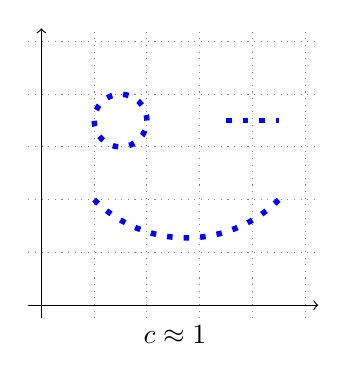
\begin{tikzpicture}[scale=0.67]
% draw the grid
\draw[->] (0,-0.25) -- (0,5.25) ;
\draw[->] (-0.25,0) -- (5.25,0) ;
\foreach \i in {1,...,5} {
    \draw[dotted,draw=gray] (-0.25,\i) -- (5.25,\i);
}
\foreach \i in {1,...,5} {
    \draw[dotted,draw=gray] (\i,-0.25) -- (\i,5.25);
}

\draw[loosely dotted,draw=blue,line width=2pt] (1,2) to[in=225,out=-45] (4.5,2);
\path[loosely dotted,draw=blue,line width=2pt] (1.5,3.5) circle (0.5);
\draw[loosely dotted,draw=blue,line width=2pt] (3.5,3.5) to (4.5,3.5);

\node[anchor=north west] at (1.75,-0.2) {$c \approx 1$};

\end{tikzpicture}
\hspace{0.5in}
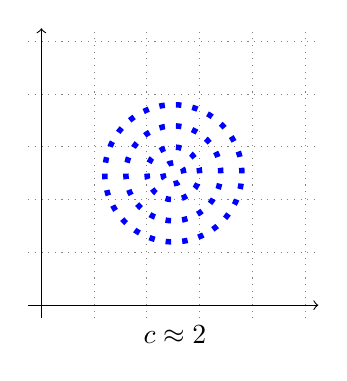
\begin{tikzpicture}[scale=0.67]
% draw the grid
\draw[->] (0,-0.25) -- (0,5.25) ;
\draw[->] (-0.25,0) -- (5.25,0) ;
\foreach \i in {1,...,5} {
    \draw[dotted,draw=gray] (-0.25,\i) -- (5.25,\i);
}
\foreach \i in {1,...,5} {
    \draw[dotted,draw=gray] (\i,-0.25) -- (\i,5.25);
}

%\draw[loosely dotted,draw=blue,line width=2pt] (1,2) to[in=225,out=-45] (4.5,2);
\path[loosely dotted,draw=blue,line width=2pt] (2.5,2.5) circle (0.2);
\path[loosely dotted,draw=blue,line width=2pt] (2.5,2.5) circle (0.5);
\path[loosely dotted,draw=blue,line width=2pt] (2.5,2.5) circle (0.9);
\path[loosely dotted,draw=blue,line width=2pt] (2.5,2.5) circle (1.3);
%\draw[loosely dotted,draw=blue,line width=2pt] (3.5,3.5) to (4.5,3.5);

\node[anchor=north west] at (1.75,-0.2) {$c \approx 2$};

\end{tikzpicture}
\end{center}

%\textbf{Theorem:} In any Euclidean space $\R^d$, the doubling dimension = $O(d)$

\pause
\vspace{0.1in}
    \textbf{
$c$ small $\Rightarrow$ lots of structure; $c$ large $\Rightarrow$ little structure
}

\end{frame}

%%%%%%%%%%%%%%%%%%%%%%%%%%%%%%%%%%%%%%%%%%%%%%%%%%%%%%%%%%%%%%%%%%%%%%%%%%%%%%%%

\begin{frame}{The doubling dimension $c$}

A set $C$ is a \textbf{$\delta$-covering} of $X$ if for all $x\in X$, there exists a $c \in C$ such that $\dist{x}{c} \le \delta$.
The \textbf{covering number} of $X$, denoted $N_\delta(X)$, is the cardinality of the smallest $\delta$-covering.
The \textbf{doubling constant} is 
\begin{equation}
2^c = \max_{x\in X,\delta>0} N_\delta( B(x,2\delta))
.
\end{equation}

%
%An \textbf{$r$-covering} of a set $X$ is a subset of $X$ such that all pairwise distances are greater than $r$. %$\{x_1,x_2,...x_M\} \subset X$ such that $\dist{x_i}{x_j} > r$ for all distinct $i,j$.
%
%The \textbf{$r$-packing number} $M_r (X)$ is the cardinality of the largest $r$-packing.
%

\vspace{0.1in}
\hrule
\vspace{0.1in}
%%%%%%%%%%%%%%%%%%%%%%%%%%%%%%%%%%%%%%%%

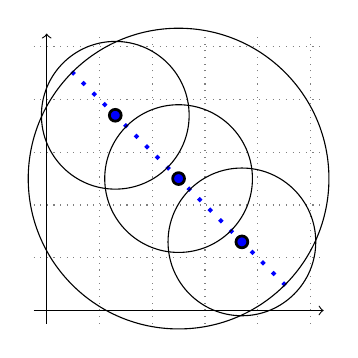
\begin{tikzpicture}[scale=0.67]
% draw the grid
\draw[->] (0,-0.25) -- (0,5.25) ;
\draw[->] (-0.25,0) -- (5.25,0) ;
\foreach \i in {1,...,5} {
    \draw[dotted,draw=gray] (-0.25,\i) -- (5.25,\i);
}
\foreach \i in {1,...,5} {
    \draw[dotted,draw=gray] (\i,-0.25) -- (\i,5.25);
}

%\foreach \i in {1,...,10} {
    %\foreach \j in {1,...,10} {
        %\node[bluedot] at (0.3*\i,0.3*\j) {};
    %}
%}
\node[bluedot] at (2.5,2.5) {};
\foreach \i in {1,...,10} {
    \node[bluedot] at (2.5+0.2*\i,2.5-0.2*\i) {};
    \node[bluedot] at (2.5-0.2*\i,2.5+0.2*\i) {};
}

\uncover<2-5> {
\node[reddot]  at (2.5,2.5) {};
\path[draw=black] (2.5,2.5) circle (1.4);
\path[draw=black] (2.5,2.5) circle (2.85);

\node[reddot]  at (1.3,3.7) {};
\path[draw=black] (1.3,3.7) circle (1.4);
\node[reddot]  at (3.7,1.3) {};
\path[draw=black] (3.7,1.3) circle (1.4);
}

\uncover<2-5> {
%\node[fill=white] at (1.5,0) {\textcolor{darkgreen}{robust}};
%\node at (2.5,-1) {\textcolor{darkgreen}{$c=O(d)$}} ;
}
\end{tikzpicture}
%%%%%%%%%%%%%%%%%%%%
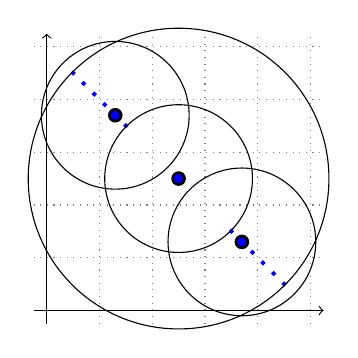
\begin{tikzpicture}[scale=0.67]
% draw the grid
\draw[->] (0,-0.25) -- (0,5.25) ;
\draw[->] (-0.25,0) -- (5.25,0) ;
\foreach \i in {1,...,5} {
    \draw[dotted,draw=gray] (-0.25,\i) -- (5.25,\i);
}
\foreach \i in {1,...,5} {
    \draw[dotted,draw=gray] (\i,-0.25) -- (\i,5.25);
}

\node[bluedot] at (2.5,2.5) {};
\foreach \i in {1,...,6} {
    \node[bluedot] at (3.3+0.2*\i,1.7-0.2*\i) {};
    \node[bluedot] at (1.7-0.2*\i,3.3+0.2*\i) {};
}

\uncover<3-5>{
\node[reddot] at (2.5,2.5) {};
\path[draw=black] (2.5,2.5) circle (1.4);
\path[draw=black] (2.5,2.5) circle (2.85);

\node[reddot]  at (1.3,3.7) {};
\path[draw=black] (1.3,3.7) circle (1.4);
\node[reddot]  at (3.7,1.3) {};
\path[draw=black] (3.7,1.3) circle (1.4);
}
\uncover<3-5> {
%\node[fill=white] at (1.5,0) {\textcolor{darkgreen}{robust}};
%\node at (2.5,-1) {\textcolor{darkgreen}{$c=O(d)$}} ;
}
\end{tikzpicture}
%%%%%%%%%%%%%%%%%%%%
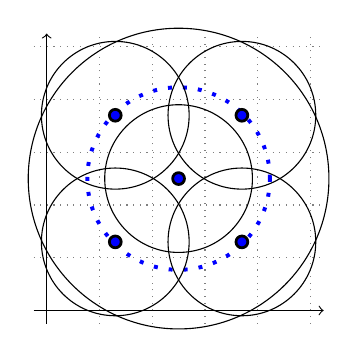
\begin{tikzpicture}[scale=0.67]
% draw the grid
\draw[->] (0,-0.25) -- (0,5.25) ;
\draw[->] (-0.25,0) -- (5.25,0) ;
\foreach \i in {1,...,5} {
    \draw[dotted,draw=gray] (-0.25,\i) -- (5.25,\i);
}
\foreach \i in {1,...,5} {
    \draw[dotted,draw=gray] (\i,-0.25) -- (\i,5.25);
}

\node[bluedot] at (2.5,2.5) {};
\path[loosely dotted,draw=blue,line width=0.5mm] (2.5,2.5) circle (1.73);

\uncover<4-5>{
\node[reddot] at (2.5,2.5) {};
\path[draw=black] (2.5,2.5) circle (1.4);
\path[draw=black] (2.5,2.5) circle (2.85);
}
\uncover<4-5>   {
\node[reddot]  at (1.3,3.7) {};
\path[draw=black] (1.3,3.7) circle (1.4);
\node[reddot]  at (3.7,3.7) {};
\path[draw=black] (3.7,3.7) circle (1.4);
\node[reddot]  at (3.7,1.3) {};
\path[draw=black] (3.7,1.3) circle (1.4);
\node[reddot]  at (1.3,1.3) {};
\path[draw=black] (1.3,1.3) circle (1.4);

    %\node[fill=white] at (1.5,0) {\textcolor{darkgreen}{robust}};
    %\node at (2.5,-1) {\textcolor{darkgreen}{$c=O(d)$}};
}
\end{tikzpicture}

%\uncover<5>{
%\vspace{-2.80in}
%\begin{tikzpicture}
%\node[fill=lightyellow,draw=black,thick,text width=11.05cm,rounded corners=0.1cm,inner sep=0.2in] at (0,0) { 
    %\textcolor{darkgreen}{Advantage: robust to all changes in the data set}
    %\\
    %\textcolor{red}{Disadvantage: cannot be used for exact nearest neighbor queries}
%};
%\end{tikzpicture}
%}
%
%\vspace{1.8in}

\end{frame}

